\chapter{Results and Future}\label{part1_results_and_future}

All objectives which we defined in \hyperref[targets]{\emph{section 1.2}} have been achieved. The optional goal to provide vector tiles for the entire world has been moved to the bachelor thesis.

\section{Results}\label{part1_results}

\begin{itemize}
\item
  Docker containers and documentation for the entire workflow of creating vector tiles has been created.
\item
  The raster tile server for serving the vector tiles together with a visual style has been realized.
\item
  The project website with information about how to use the vector tiles is online.
\end{itemize}

The vector tiles for Switzerland can be downloaded from the project website (\url{http://osm2vectortiles.org}). These vector tiles can be served together with a visual style in our vector tile server.
\newline{}
A custom visual style can be created with Mapbox Studio Classic\footnote{\url{https://www.mapbox.com/mapbox-studio-classic/}}.
All existing visual styles based of Mapbox Streets are compatible with the produced vector tiles. This allows very easy migration to osm2vectortiles.

\begin{figure}[H]
  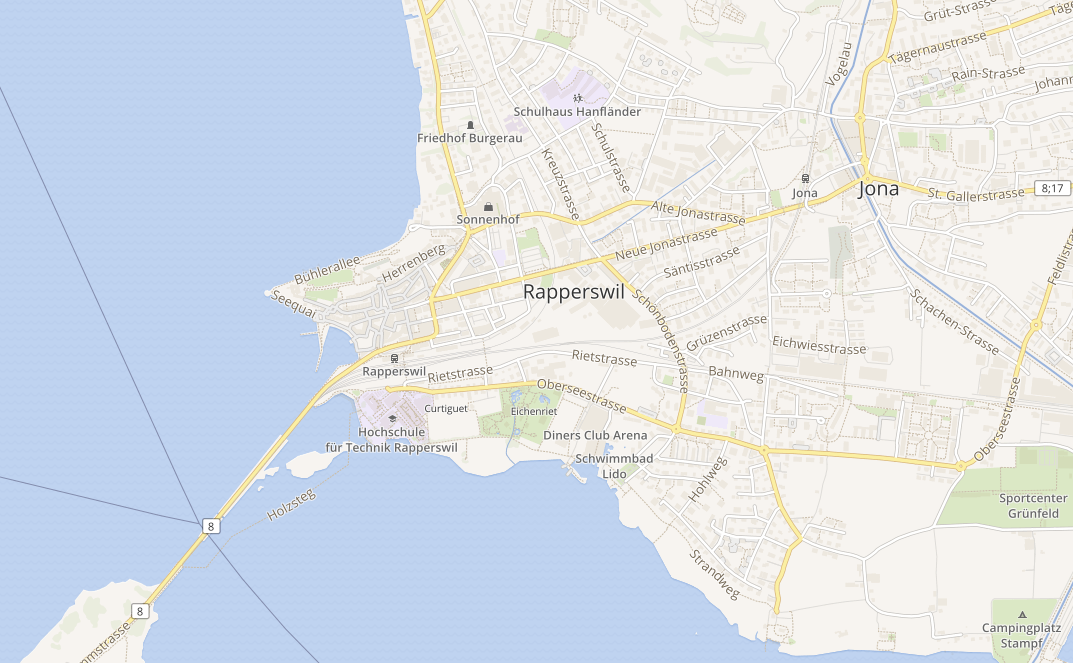
\includegraphics[width=1\textwidth]{images/unmodified_osm_bright.png}
  \caption{Unmodified OSM Bright visual style using osm2vectortiles}
\end{figure}

\section{Future}\label{part1_future}
In a first step the project should be expanded to provide vector tiles for the entire world. The vector tile rendering workflow needs to be scaled out for the entire world. Regular updates for the vector tiles have been requested by the members of the Swiss OSM community
and will require identifying and rerendering updated tiles.\\
The long-term vision of this project is to provide a complete offline map experience, including basic geographic name search. These suggestions will be the project goals for the bachelor thesis. More detailed listing of
future features can be found in \autoref{part2_results_and_future}.
